\section{Analizando la complejidad temporal}

\subsection{Obtención del maximo}
Dada la observación al inicio del informe se sabe que las listas de entrada de esfuerzo y energia cumplen con $\lvert E_i \lvert \ = \lvert S_j \lvert$ por lo tanto en un principio se tendría rapidamente y sin profundizar que:

$$
T(n) = O(n²) \text{ siendo n el tamaño de cualquiera de las dos entradas}
$$

En un principio observamos el comportamiento del algoritmo para algunos elementos y observamos la curva de medicion empìrica:

\begin{figure}[H]
    \centering
    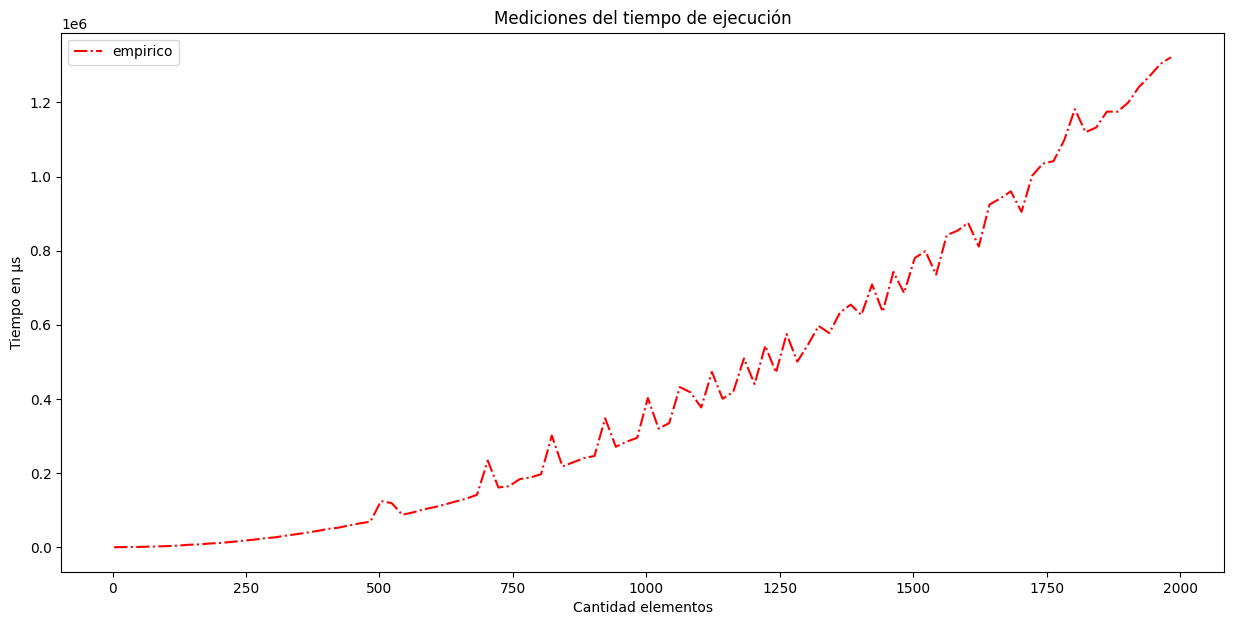
\includegraphics[width=1\textwidth]{graficos/tiemposejecucion.png}
\end{figure}

En la grafica anterior podemos observar la duración en microsegunos del tiempo de ejecución del algoritmo para un conjunto de datos aleatorios en el rango de cero y dos mil elemenos

Por otro lado, se realiza una curva teorica de la complejidad, del tipo cuadratica que resulta de elevar al cuadrado la longitud del cardinal de alguno de los dos conjuntos 

\begin{figure}[H]
    \centering
    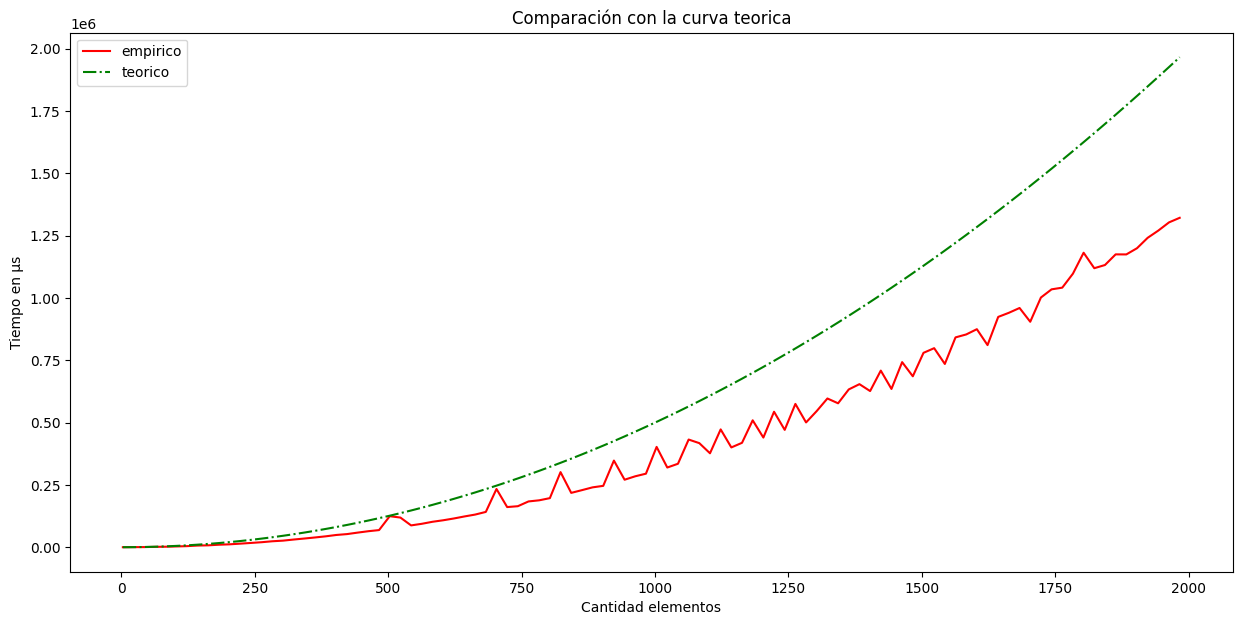
\includegraphics[width=1\textwidth]{graficos/vsteorica.png}
\end{figure}

La grafica contiene la medicion anteriormente realizada pero esta vez se compara tambien contra un tiempo teorico estimado, en un principio pareceria que el algoritmo se encuentra correctamente acotado por el tiempo teorico.

Ahora es importante analizar otros aspectos del problema, se debe verificar que este no tenga un comportamiento diferente respecto la longitud en bits de la entrada, en otras palabras, habra que verificar si este algoritmo cumple o no con ser de caracter pseudopolinomial

Analicemos primero como se comporta la longitud en bits del tamaño de la entrada, es importante ver que la longitud en bits del tamaño de la entrada va a ser constante en determinados rangos, y dando un ejemplo de esto, para 8 y 10 necesito la misma cantidad de bits para representarlos dentro del computador, esto es pues que necesito $\log_2(n)
$ digitos para representar el valor. Como en el dominio del problema siempre voy a tener que la longitud de la entrada es igual para cada conjunto, la variabilidad segun esta crece no es significativa para el problema y esto significa que para determinados rangos de los valores de entrada el generar la matriz del espacio de solución puede verse como una constante. 

Para validar dicha idea, hace falta realizar una grafica en escala logaritmica (por un tema de comodidad) en donde se grafica la longitud en bits de la entrada en contra del logaritmo de la medición realizada anteriormente, en caso de encontrar que estos datos se comportan de manera lineal en la escala, se habra determinado empiricamente que dicho algoritmo es de caracter pseudopolinomial. Y por lo tanto seria una prueba para eliminar la cota teorica anteriormente planteada

\begin{figure}[H]
    \centering
    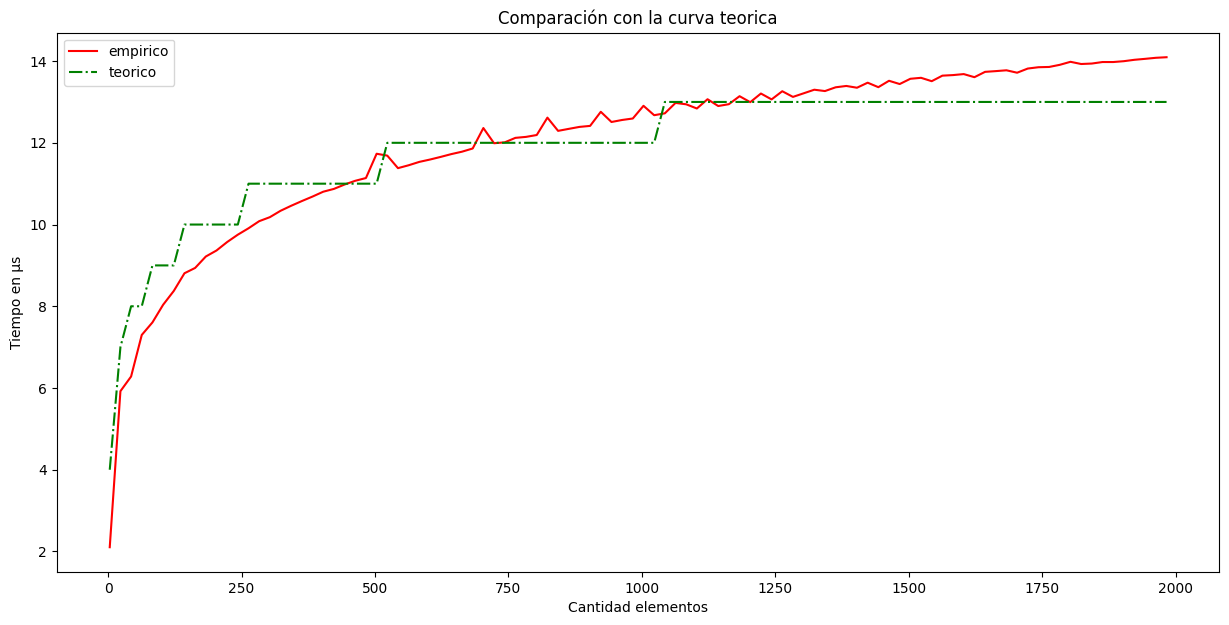
\includegraphics[width=1\textwidth]{graficos/logaritmica.png}
\end{figure}

La grafica anterior, sirve como un metodo empirico para refutar un supuesto comportamiento pseudopolinomial del algoritmo. Por lo tanto la cota temporal en notación Big O obtenida en un principio sigue sostenida por las pruebas de medición realizadas en el analisis. Finalmente se afirma con mayor criterio que:

$$
 T(n) = O(n²)
$$

Donde L es la longitud de la entrada del esfuerzo o la energia 

\subsection{Reconstrucción de secuencia}
Reconstruir la secuencia depende de dos cosas: 

- Encontrar la posicion de un maximo en un arreglo
- Iterar k + 1 veces cada vez que la recurción llega a una fila nueva 

En este caso, se genero una funcion que hace  $T(n) = O(n)$, por otro lado, iterar k + 1 veces tambien cumple con ser lineal $T(n) = O(n)$.

En un principio dicho algoritmo para un caso generico parece ser también cumplir con ser $T(n) = O(n)$

Hay un gran pero en la complejidad anteriormente asignada, existe la posibilidad de que la secuencia de entrenamiento llegue a ser una secuencia alternada $(Entrenamiendo, Descanso, Entrenamiendo, ...)$, entonces se sabe que este algoritmo buscara la posicion del maximo un aproximado de $n/2$ lo cual es hacer algo lineal $n/2$ veces que se aproxima más a un caso cuadratico (se descartan las iteraciones realizadas en la reconstrucción de la secuencia porque son siempre de longitud 1), ahora como es muy particular podemos definir un comportamiento general y un peor caso. 

Entonces este algoritmo se comportaria de la siguiente manera:

$$
T(n) = O(n) \text{ para casos generales} \\
$$
T(n) = O(n^2) \text{ para el caso de tener una secuencia que sea siempre alternada} \\
$$
 \text{ siendo n la longitud de cualquier fila del espacio de solución}
$$

Se agrega una grafica con las mediciones temporales del algoritmo para comprobar su comportamiento estimado

\begin{figure}[H]
    \centering
    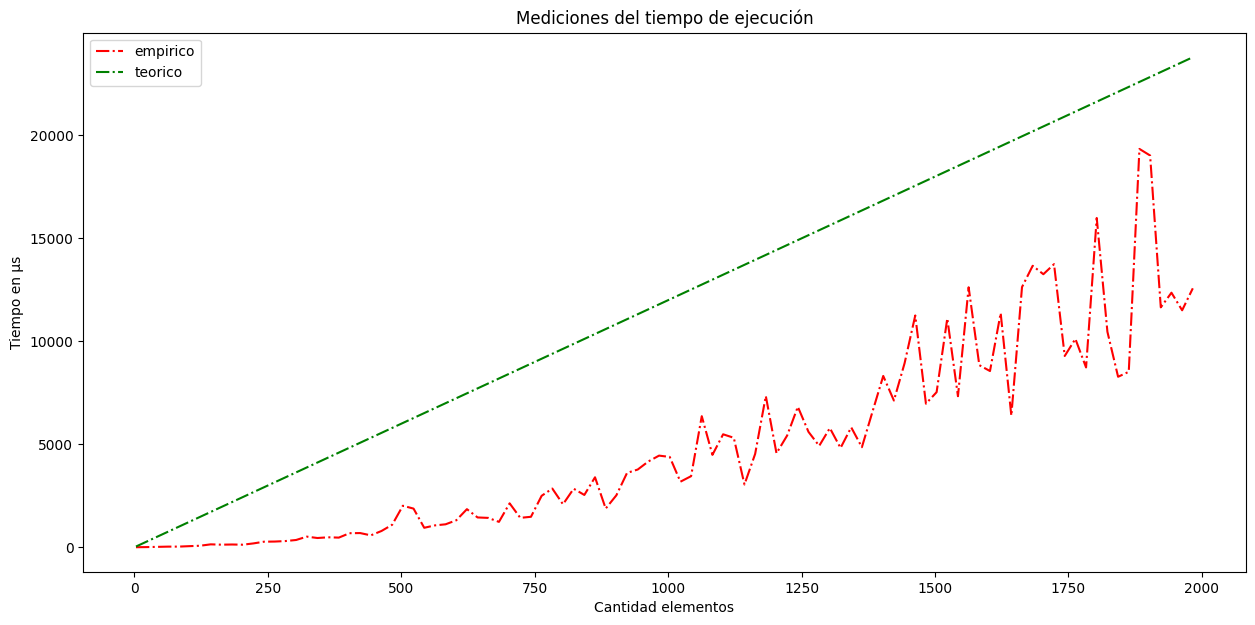
\includegraphics[width=1\textwidth]{graficos/reconstruccion.png}
\end{figure}

En esta grafica se puede comprobar que el comportamiendo del algoritmo tiene una tendencia de creciento lineal, tal como se estimaba, asi como tambien que la velocidad varia bastante dependiendo de la cantidad de saltos "descansos" que tenga la secuencia de entrenamiento. 